%%%%%%%%%%%%%%%%%%%%%%%%%%%%%%%%%%%%%%%%%%%%%%%%%%%%%%%%%%%%%%%%%%%%%
%
%	Copyright 2014 Jean-Philippe Eisenbarth
%		Original template from:
%		https://github.com/Eisenbarth/SRS-Tex
%
%	Copyright 2016 Simone Bisi
%		Riadattato per il corso "Linguaggi Dinamici"
%		presso Università degli studi di Modena e Reggio Emilia
%
%%%%%%%%%%%%%%%%%%%%%%%%%%%%%%%%%%%%%%%%%%%%%%%%%%%%%%%%%%%%%%%%%%%%%

\documentclass{scrreprt}

%%%%%%%%%%%%%%%%%%%%%%%%%%%%%%%%%%%%%%%%%%%%%%%%%%%%%%%%%%%%%%%%%%%%%

\usepackage{listings}
\usepackage{underscore}
\usepackage[bookmarks=true]{hyperref}
\usepackage[utf8]{inputenc}
\usepackage[italian]{babel}
\usepackage{afterpage}

\usepackage{makeidx}
\usepackage{hyperref}
\usepackage{bookmark}

\usepackage{placeins}
\usepackage{multirow}

\usepackage{listings}

\usepackage{graphicx}
\graphicspath{ {images/} }

% Default fixed font does not support bold face
\DeclareFixedFont{\ttb}{T1}{txtt}{bx}{n}{12} % for bold
\DeclareFixedFont{\ttm}{T1}{txtt}{m}{n}{12}  % for normal

% Custom colors
\usepackage{color}
\definecolor{deepblue}{rgb}{0,0,0.5}
\definecolor{deepred}{rgb}{0.6,0,0}
\definecolor{deepgreen}{rgb}{0,0.5,0}

\usepackage{listings}

% Python style for highlighting
\newcommand\pythonstyle{\lstset{
language=Python,
basicstyle=\ttm,
otherkeywords={self},             % Add keywords here
keywordstyle=\ttb\color{deepblue},
emph={MyClass,__init__},          % Custom highlighting
emphstyle=\ttb\color{deepred},    % Custom highlighting style
stringstyle=\color{deepgreen},
frame=tb,                         % Any extra options here
showstringspaces=false            % 
}}


% Python environment
\lstnewenvironment{python}[1][]
{
\pythonstyle
\lstset{#1}
}
{}

% Python for external files
\newcommand\pythonexternal[2][]{{
\pythonstyle
\lstinputlisting[#1]{#2}}}

% Python for inline
\newcommand\pythoninline[1]{{\pythonstyle\lstinline!#1!}}

\makeindex

%%%%%%%%%%%%%%%%%%%%%%%%%%%%%%%%%%%%%%%%%%%%%%%%%%%%%%%%%%%%%%%%%%%%%

\def \author 	{Simone Bisi}
\def \project 	{Sito per l'ordinamento di\\immagini tramite\\crowdsourcing}
\def \from		{Università degli studi di Modena\\e Reggio Emilia}
\def \class 	{Linguaggi Dinamici}

\hypersetup{
    bookmarks=false,    								% bookmarks
    pdftitle={Crowdfight},    							% title
    pdfauthor={\author},	                     		% author
    pdfsubject={Gummi 0.6.5 and LaTeX},    				% subject
    pdfkeywords={}, 	% list of keywords
    colorlinks=true,    % false: boxed links; true: colored links
    linkcolor=blue,     % color of internal links
    citecolor=black,    % color of links to bibliography
    filecolor=black,    % color of file links
    urlcolor=purple,    % color of external links
    linktoc=page        % only page is linked
}
\date{}

%%%%%%%%%%%%%%%%%%%%%%%%%%%%%%%%%%%%%%%%%%%%%%%%%%%%%%%%%%%%%%%%%%%%%

\begin{document}

\begin{flushright}
    \rule{16cm}{5pt}\vskip1cm
    \begin{bfseries}
        \Huge{Progetto sviluppato mediante framework Django}\\
        \vspace{1.9cm}
        per\\
        \vspace{1.9cm}
        {\normalfont{\textit{\project}}}
        {\textsc{ }}\\
        \LARGE\vspace{1.9cm}
        di \author\\
        \vspace{0.5cm}
        \textsc{\from}\\
        {\normalfont{Corso di \textit{\class}}}\\
        \vspace{2.0cm}
        \today\\
    \end{bfseries}
\end{flushright}

%%%%%%%%%%%%%%%%%%%%%%%%%%%%%%%%%%%%%%%%%%%%%%%%%%%%%%%%%%%%%%%%%%%%%

\newcommand\blankpage{%
    \null
    \thispagestyle{empty}%
    \addtocounter{page}{-1}%
    \newpage}

\null
\addtocounter{page}{-1}%
\thispagestyle{empty}%
\blankpage{}

%%%%%%%%%%%%%%%%%%%%%%%%%%%%%%%%%%%%%%%%%%%%%%%%%%%%%%%%%%%%%%%%%%%%%

\tableofcontents

%%%%%%%%%%%%%%%%%%%%%%%%%%%%%%%%%%%%%%%%%%%%%%%%%%%%%%%%%%%%%%%%%%%%%

\chapter{Introduzione}

\section{Obiettivo}
Il seguente documento ha lo scopo di illustrare la creazione di un sito per l'ordinamento delle immagini
seguendo il metodo del \textit{crowdsourcing}. Questo metodo è già stato applicato con successo da siti web come KittenWar (\textit{www.kittenwar.com}) e PuppyWar (\textit{www.puppywar.com}).

%====================================================================

\section{Fonti}
%Elenco completo di tutte le fonti (documenti, libri, siti, altro)
Il progetto è stato elaborato partendo dalle specifiche della traccia fornite dalla docente e completato con ipotesi ragionevoli per tutto ciò che non è specificato nel testo iniziale, di seguito riportato.
\begin{quote}
Creare uno sito sullo stile di kittenwar (www.kittenwar.com) che propone un approccio di tipo
crowdsourcing per l'ordinamento di immagini su un tema specifico.
In pratica, si parte da un set prefissato di immagini in cui ogni immagine è associata ad un
punteggio. Ciascun utente che accede al sito vede due immagini selezionate casualmente. Per
ciascuna coppia, l'utente deve decidere l'immagine vincente: il vincitore vede il proprio punteggio
aumentato di 1/n, mentre il perdente vede il proprio punteggio diminuito di 1/n, dove n e' il numero
di competizioni fino a quel momento sostenute dall'immagine
Utenti:
- Gli utenti anonimi possono votare le immagini e visualizzare diversi tipi di informazioni sulle
classifiche (vedere sotto)
- Gli utenti registrati possono aggiungere nuove immagini al dataset: le nuove immagini che
vengono aggiunte in fasi successive devono iniziano con un punteggio che li pone nella parte
intermedia delle classifica. Possono inoltre visualizzare statistiche relative alle immagini da essi
stessi caricate.
Informazioni visualizzabili da utenti anonimi: lista delle immagini "piu vincenti" e "piu' perdenti"
(testa e la coda della
 classifica attuali), l'immagine vincitrice di una certa giornata o settimana.
Statistiche che è possibile visualizzare da parte di utenti registrati: definire almeno tre statistiche di
interesse (es. percentuale delle immagini caricate che sono risultate vincitrici per una data giornata).
Facoltativo: valutare algoritmi di selezione delle immagini piu' raffinati, per esempio facendo
scontrare tra di loro immagini con punteggi vicini, oppure algoritmi che cercano di mantenere
simile il numero di match sostenuti da ciascuna immagine
\end{quote}
Questo documento riassuntivo è stato realizzato mediante l'utilizzo del linguaggio di markup \LaTeX\\ e compilato in PDF mediante l'editor \textit{Gummi}.

%%%%%%%%%%%%%%%%%%%%%%%%%%%%%%%%%%%%%%%%%%%%%%%%%%%%%%%%%%%%%%%%%%%%%
%%%%%%%%%%%%%%%%%%%%%%%%%%%%%%%%%%%%%%%%%%%%%%%%%%%%%%%%%%%%%%%%%%%%%
%%%%%%%%%%%%%%%%%%%%%%%%%%%%%%%%%%%%%%%%%%%%%%%%%%%%%%%%%%%%%%%%%%%%%

\chapter{Descrizione generale}

Il progettto sviluppa un sito web denominato \textit{Crowdfight} (derivato dalla parola \textit{crowdsourding}) orientato all'ordinamento di un set di immagini da parte degli utenti.\\
Viene proposto un approccio del tipo "sfida" tra due immagini alla volta e, basandosi sulla scelta dell'utente, si può stilare una classifica di immagini più o meno preferite.

%--------------------------------------------------------------------

\section{Interfaccia utente (\textit{frontend})}

\subsection{Struttura generale}

\newcounter{countStr}
\newcommand{\structure}{\stepcounter{countStr}\thecountStr}

\FloatBarrier
\begin{table}[h|]
\centering
\begin{tabular}{|l|l|p{10cm}|}
\hline
 & \textbf{Pagina HTML} & \textbf{Funzione} \\ \hline
\structure & \textit{base.html} & Template HTML genitore di tutte le altre pagine \\ \hline
\structure & \textit{add_image.html} & Form per caricare una nuova immagine sul sito (solo per utenti registrati) \\ \hline
\structure & \textit{ratings.html} & Pagina orientata alla visualizzazione delle classifiche (si veda la sezione \textit{Visualizzazione delle classifiche}) \\ \hline
\structure & \textit{image.html} & Pagina orientata alla visualizzazione di una singola immagine (si veda la sezione \textit{Visualizzazione di un'immagine}) \\ \hline
\structure & \textit{top_day.html} & Pagina orientata alla visualizzazione delle migliori immagini dei giorni passati  \\ \hline
\structure & \textit{stats.html} & Pagina per la visualizzazione delle statistiche personali (solo per utenti registrati)\\ \hline
\structure & \textit{register.html} & Pagina di registrazione utente \\ \hline
\structure & \textit{profile.html} & Pagina del profilo di un utente \\ \hline
\structure & \textit{login.html} & Pagina di login \\ \hline
\structure & \textit{index.html} & Pagina iniziale \\ \hline
\end{tabular}
\end{table}
\FloatBarrier

\subsection{Pagina iniziale}
Il sito web si presenta, sia agli utenti anonimi che a quelli registrati, con un'interfaccia che presenta loro due immagini scelte in modo casuale dal database.
\\\\
\centerline{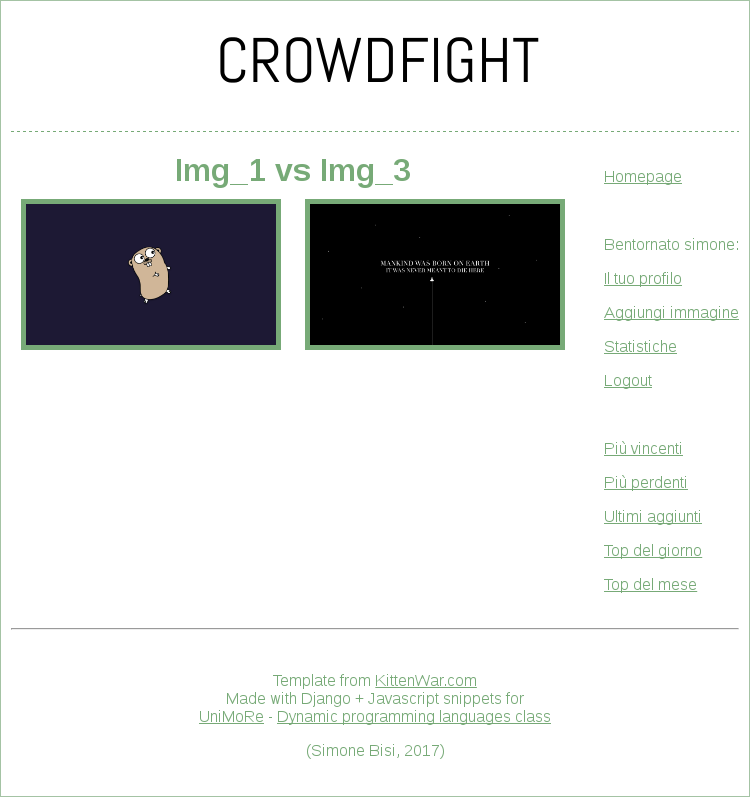
\includegraphics[scale=0.40]{front}}
\\\\
In base alla scelta dell'utente tramite JavaScript viene impostato un cookie che memorizza quale immagine è stata votata. Il framework Django ottiene tale cookie dalla variabile \textit{request} e mostra nella pagina di risposta un resoconto delle sfide vinte da ciascuna immagine.\\

\centerline{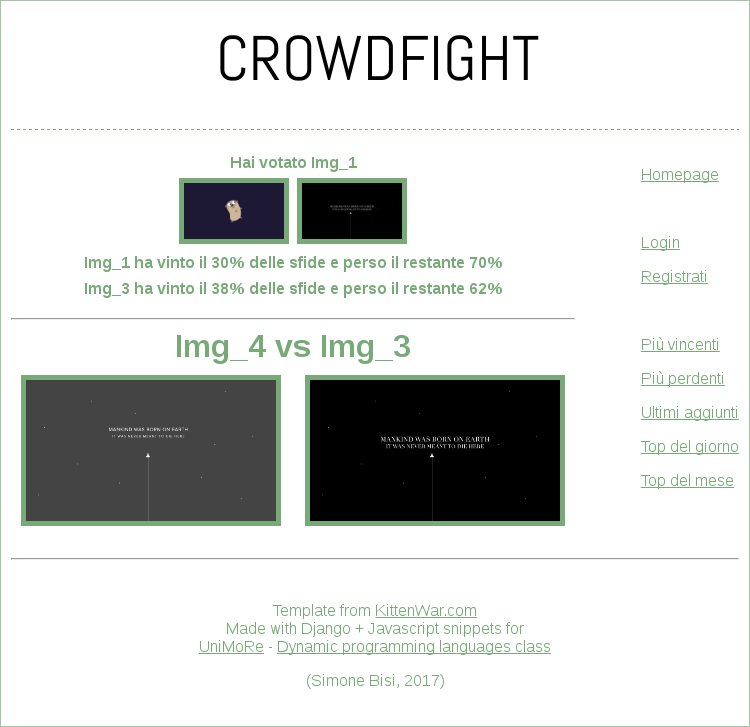
\includegraphics[scale=0.40]{vote}}

\pagebreak

\subsection{Profilo di un utente}
Le pagine del profilo di un utente sono visualizzabili da qualsiasi utente. La pagina informa il visitatore se si tratta di un utente appartenente al gruppo staff e mostra l'email solo nel caso si tratti della propria pagina utente.
Si è scelto di utilizzare il modello \textit{User} predefinito di Django in quanto non è stato necessario aggiungere nessun campo personalizzato a quelli già esistenti.\\
Tra i campi visualizzati in modo pubblico si trovano la data dell'ultimo accesso e la data di registrazione.
Vengono inoltre mostrate tutte le immagini caricate dall'utente.
\\\\
\centerline{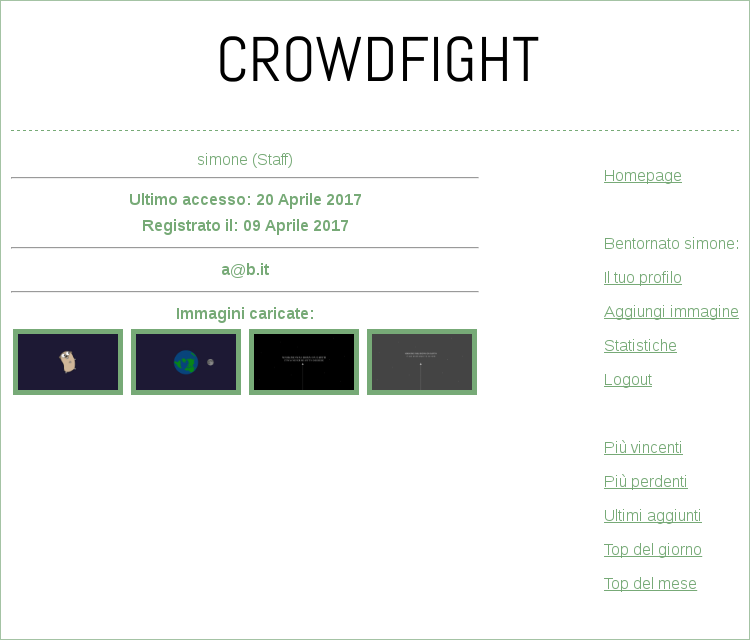
\includegraphics[scale=0.46]{profile}}
\\\\

\pagebreak

\subsection{Visualizzazione di un'immagine}
Il sito utilizza una gerarchia di \textit{view} per la visualizzare la descrizione di una singola immagine.
\\\\
\centerline{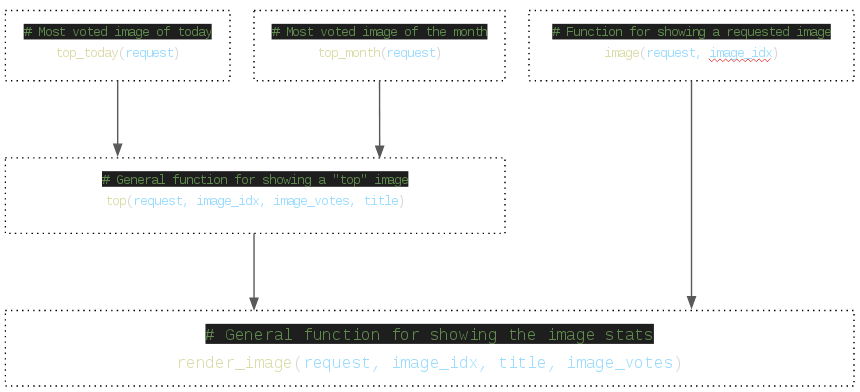
\includegraphics[scale=0.46]{schemeimg}}
\\\\La funzione \textit{render_image} provvede poi ad caricare i dati dell'immagine richiesta e calcolare le varie percentuali di vittorie e sconfitte. È possibile cancellare l'immagine se essa appartiene all'utente che la sta visualizzando.\\
Tramite \textit{JavaScript} a livello client viene mostrato un form che permette di confermare o annullare l'eliminazione.
\\\\
\centerline{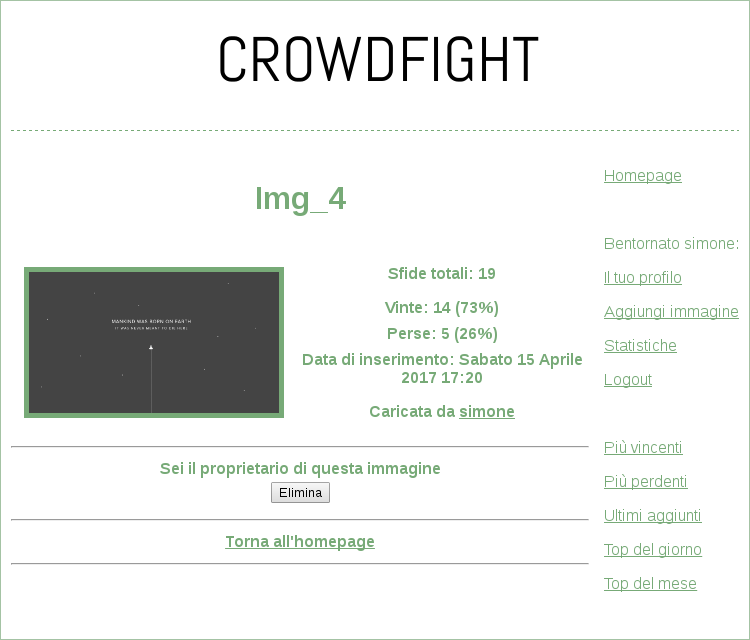
\includegraphics[scale=0.46]{single}}
\pagebreak

\subsection{Visualizzazione delle classifiche}
Le pagine riguardanti la parte iniziale e finale della classifica (immagini migliori e peggiori di sempre) e le ultime 10 inserite vengono visualizzate, analogamente alle immagini singole, tramite una \textit{view} più generica in modo che l'unica funzione \textit{ratings} si occupi di visualizzare l'array di immagini che gli viene fornito in ingresso, calcolando tutte le percentuali desiderate.\\\\
\centerline{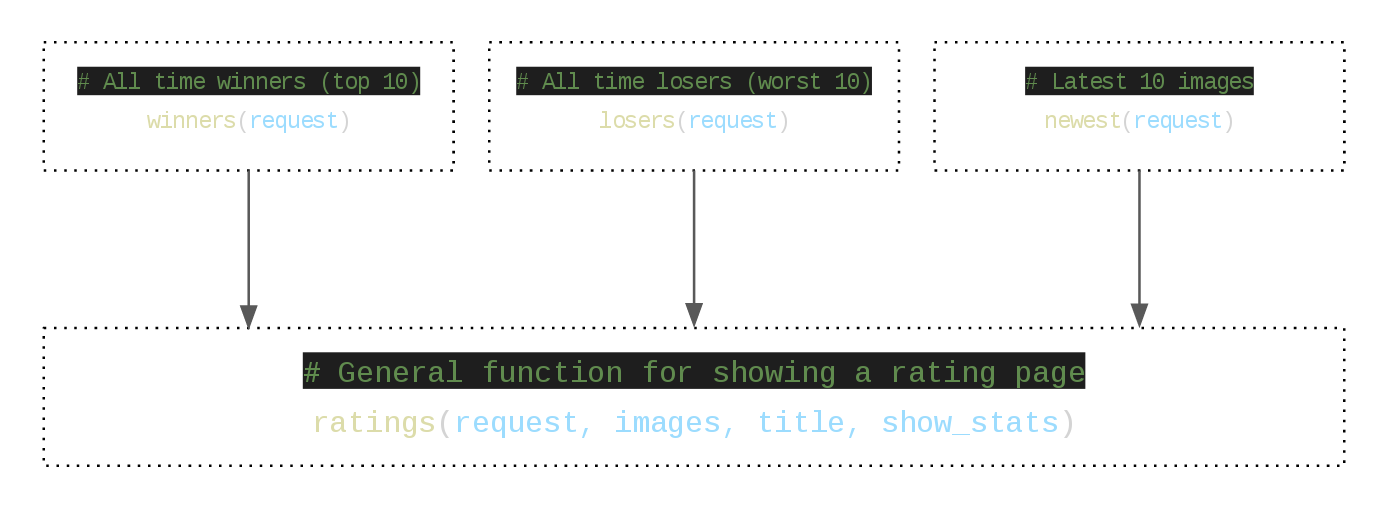
\includegraphics[scale=0.33]{schemeratings}}
In tutte le pagine è possibile selezionare quante immagini si vogliono visualizzare tramite un \textit{form} a tendina.\\\\
\centerline{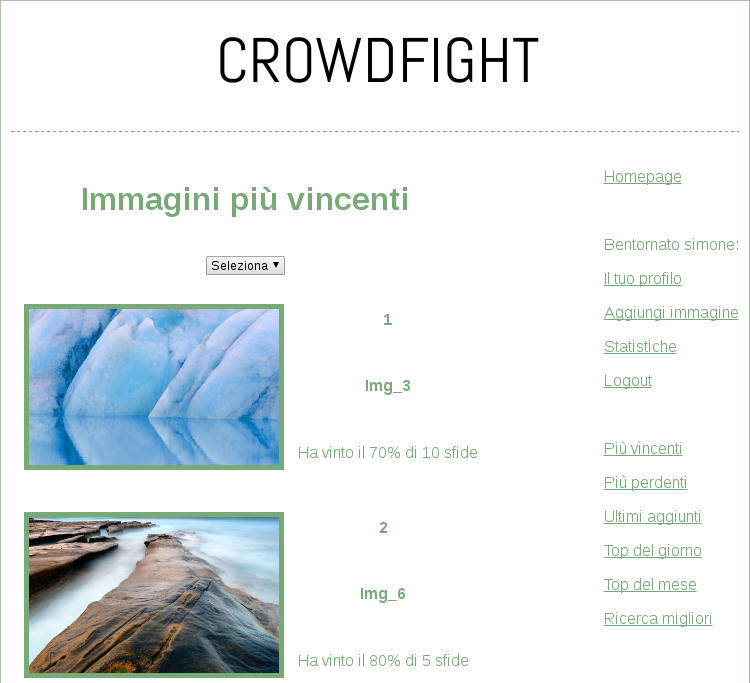
\includegraphics[scale=0.38]{ratings}}
\pagebreak

\subsection{Statistiche per utenti registrati}
Tramite registrazione al sito è inoltre possibile accedere ad una pagina riservata che permette di visualizzare statistiche personalizzate sulle sfide sostenute dalle proprie immagini. Tramite menù a tendina si possono selezionare le proprie immagini e tramite due form input di tipo \textit{date} (forniti da HTML5) si può selezionare l'intervallo di date su cui effettuare la ricerca.\\
I grafici, generati utilizzando la libreria \textit{django-graphos} che funge da API Python per gestire in modo agevole il servizio web \textit{Google Charts}, ragruppano sull'asse orizzontale le vittore e le sconfitte ottenute da un'immagine in una determinato giorno. 
\\\\
\centerline{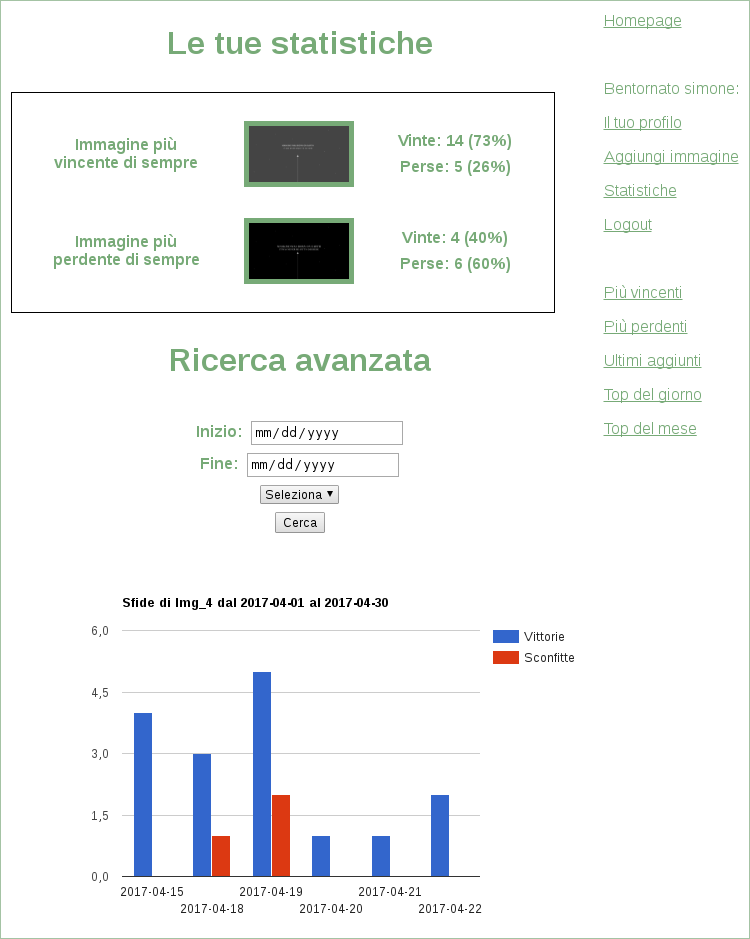
\includegraphics[scale=0.46]{stats}}
\pagebreak

\subsection{Caricamento di una nuova immagine}
Un utente registrato può caricare in qualsiasi momento una nuova immagine tramite un semplice form di caricamento.\\\\
\centerline{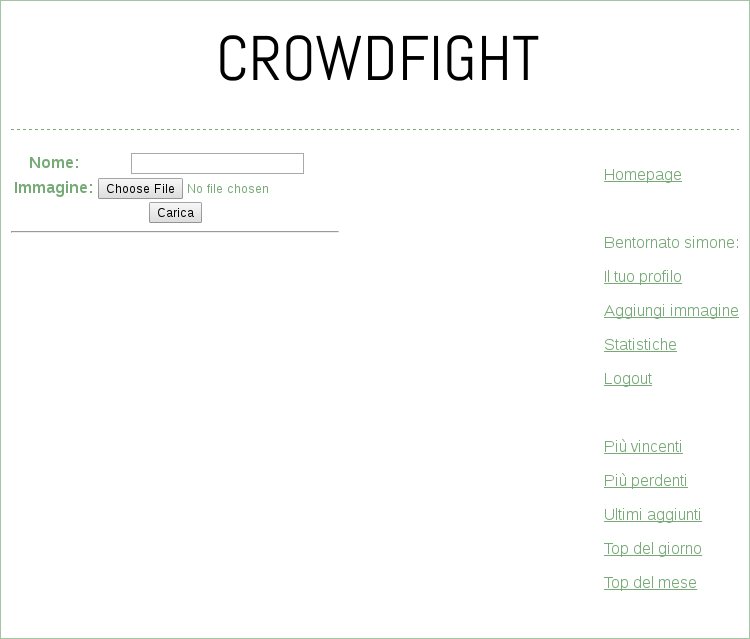
\includegraphics[scale=0.46]{upload}}
\\\\
Al momento del caricamento dell'immagine avviene la generazione dell'hash SHA-1 del file. Tramite questo meccanismo è possibile prevenire l'upload di immagini duplicate.
\\\\
\centerline{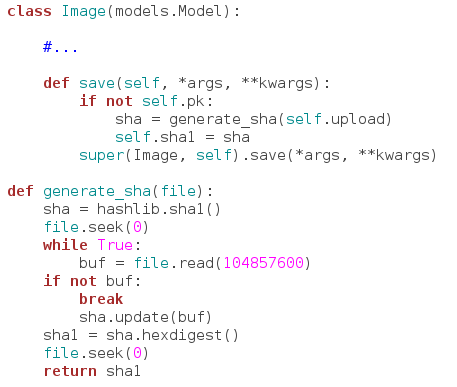
\includegraphics[scale=0.40]{codehash}}
\pagebreak

\subsection{Ricerca migliori immagini per giorni}
La pagina di ricerca delle migliori immagini permette di selezionare una ricerca orientata a cercare le immagini che hanno ricevuto più voti in ciascuna giornata fino a \textit{n} giorni prima di oggi.\\
Il numero di giorni viene automaticamente limitato a 100.
\\\\
\centerline{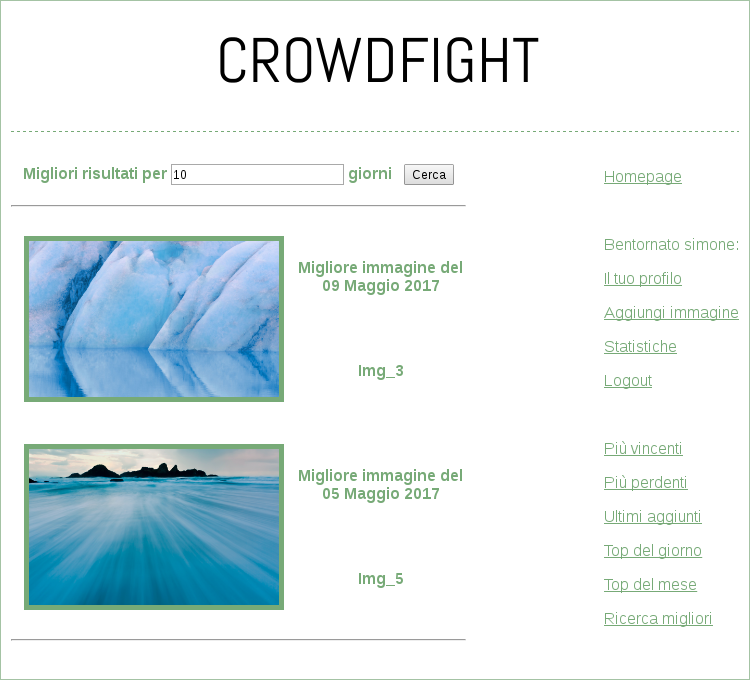
\includegraphics[scale=0.43]{topdays}}
\pagebreak

%--------------------------------------------------------------------

\section{Interfaccia di amministrazione (\textit{backend})}

Sono state aggiunte le colonne indicanti data di pubblicazione ed autore nella visualizzazione delle immagini modificando il campo \textit{list_display}.\\
È stata implementata la modalità di ricerca inserendo il campo \textit{search_fields} relativamente ai soli nomi delle immagini.\\
Si è scelto di non utilizzare affatto il modello di gruppo offerto dal framework Django, quindi lo si è rimosso dal pannello di amministrazione tramite la funzione \textit{admin.site.unregister} nel modulo \textit{admin.py}.

%--------------------------------------------------------------------

\chapter{Installazione}

\section{Dipendenze}

\textit{Crowdfight} fa uso dei seguenti pacchetti Python, disponbili con licenza \textit{open source}:
\\
\begin{itemize}
	\item
		\begin{lstlisting}
Django >= 1.8
(https://www.djangoproject.com/)
		\end{lstlisting}
		
	\item
		\begin{lstlisting}
django-graphos >= 0.3.41
(https://github.com/agiliq/django-graphos)
		\end{lstlisting}
\end{itemize}
\textit{ }\\
È possibile installare tutte le dipendenze in modo veloce tramite il package manager \textit{pip}:

\begin{lstlisting}
     sudo pip install -r requirements.txt
\end{lstlisting}

%====================================================================

\section{Procedimento}

\begin{enumerate}
\item Installare le dipendenze

\item Copiare l'app \textit{crowdfight} nel nuovo progetto

\item Aggiungere \textit{crowdfight} e \textit{graphos} alle applicazioni in \textit{settings.py}
\begin{python}
     INSTALLED_APPS = [
     	...
     	'graphos',
     	'crowdfight'
     ]
\end{python}

\item Modificare gli \textit{ALLOWED_HOSTS} in modo da permettere l'accesso al sito
\item Modificare le impostazioni di internazionalizzazione
\begin{python}
     LANGUAGE_CODE = 'it-it'
     TIME_ZONE = 'CET'
     USE_I18N = True
     USE_L10N = True
     USE_TZ = True
\end{python}

\item È necessario modificare il serializer per rendere le immagini \textit{JSON serializable}
\begin{python}
     SESSION_SERIALIZER =
     'django.contrib.sessions.serializers.PickleSerializer'
\end{python}

\item Modificare i path dei file statici e multimediali
\begin{python}
     STATIC_ROOT = BASE_DIR + '/crowdfight/static/'
     STATIC_URL = '/static/'
     MEDIA_URL = 'media/'
     LOGIN_URL = '/login'
     LOGIN_REDIRECT_URL = '/'
\end{python}

\item Aggiungere gli URL di \textit{crowdfight} in \textit{urls.py}
\begin{python}
     from django.conf.urls import include, url
     ...
     urlpatterns = [
     	...
     	url(r'^', include('crowdfight.urls'))
     ]
\end{python}

\item Effettuare la migrazione del database
\begin{python}
python manage.py makemigrations crowdfight
python manage.py migrate
\end{python}

\item Avviare il server
\begin{python}
python manage.py runserver
\end{python}

\end{enumerate}

%%%%%%%%%%%%%%%%%%%%%%%%%%%%%%%%%%%%%%%%%%%%%%%%%%%%%%%%%%%%%%%%%%%%%
%%%%%%%%%%%%%%%%%%%%%%%%%%%%%%%%%%%%%%%%%%%%%%%%%%%%%%%%%%%%%%%%%%%%%
%%%%%%%%%%%%%%%%%%%%%%%%%%%%%%%%%%%%%%%%%%%%%%%%%%%%%%%%%%%%%%%%%%%%%

\chapter{Conclusione}

L'applicazione realizzata è di facile installazione e l'interfaccia risulta di immediata comprensione per gli utenti a cui è rivolta.\\
L'interfaccia di amministrazione e l'efficente utilizzo del modello User fornito da Django mostrano come sia semplice realizzare utili applicazioni web basandosi su questo framework web gratuito ed open-source. \\
Eventuali pagine aggiuntive, statistiche e funzionalità possono essere aggiunte con facilità modificando il file \textit{views.py} e/o aggiungendo nuovi template scritti tramite HTML e linguaggio template Django.

%%%%%%%%%%%%%%%%%%%%%%%%%%%%%%%%%%%%%%%%%%%%%%%%%%%%%%%%%%%%%%%%%%%%%
%%%%%%%%%%%%%%%%%%%%%%%%%%%%%%%%%%%%%%%%%%%%%%%%%%%%%%%%%%%%%%%%%%%%%
%%%%%%%%%%%%%%%%%%%%%%%%%%%%%%%%%%%%%%%%%%%%%%%%%%%%%%%%%%%%%%%%%%%%%

% Pagina intenzionalmente bianca
\pagebreak
\blankpage{}

\end{document}
